\documentclass[12pt, letterpaper]{article}

% ——— Packages ———————————————————————————————————————————————————
\usepackage[margin=1in]{geometry}
\usepackage{graphicx}
\usepackage{amsmath, amssymb}
\usepackage{booktabs}
\usepackage{hyperref}
\usepackage{xcolor}
\usepackage{titlesec}
\usepackage{enumitem}
\usepackage{array}
\usepackage{tabularx}
\usepackage{fancyhdr}
\usepackage{float}
\usepackage{tcolorbox}
\usepackage{parskip}
\usepackage{microtype}
\usepackage{subcaption}

% ——— Colors ———————————————————————————————————————————————————————
\definecolor{accent}{RGB}{0, 180, 150}
\definecolor{accent2}{RGB}{255, 159, 67}
\definecolor{accent3}{RGB}{84, 160, 255}
\definecolor{lightgray}{RGB}{245, 250, 248}
\definecolor{darkgray}{RGB}{80, 80, 100}
\definecolor{green}{RGB}{39, 174, 96}
\definecolor{red}{RGB}{231, 76, 60}

% ——— Hyperref ————————————————————————————————————————————————————
\hypersetup{
    colorlinks=true,
    linkcolor=accent,
    urlcolor=accent,
    citecolor=accent3,
}

% ——— Header / Footer ————————————————————————————————————————————
\pagestyle{fancy}
\fancyhf{}
\rhead{\textcolor{darkgray}{\small CS 5330 \(\cdot\) Computer Vision \& Pattern Recognition}}
\lhead{\textcolor{darkgray}{\small \textbf{\textcolor{accent}{Sync}Guard}}}
\cfoot{\textcolor{darkgray}{\thepage}}
\renewcommand{\headrulewidth}{0.4pt}

% ——— Section Formatting ——————————————————————————————————————————
\titleformat{\section}{\large\bfseries\color{accent}}{}{0em}{}[\titlerule]
\titleformat{\subsection}{\normalsize\bfseries\color{darkgray}}{}{0em}{}

% ——— tcolorbox Styles ——————————————————————————————————————————
\tcbuselibrary{skins, breakable}

\newtcolorbox{infobox}[2][]{
  colback=lightgray, colframe=accent, coltitle=white,
  fonttitle=\bfseries\small, title=#2, rounded corners, #1
}
\newtcolorbox{resultbox}[2][]{
  colback=accent3!8, colframe=accent3, coltitle=white,
  fonttitle=\bfseries\small, title=#2, rounded corners, #1
}
\newtcolorbox{notebox}{
  colback=yellow!8, colframe=orange!60, rounded corners,
}

% ————————————————————————————————————————————————————————————————
\begin{document}
% ————————————————————————————————————————————————————————————————

% ——— Title Page ——————————————————————————————————————————————————
\begin{titlepage}
  \centering
  \vspace*{1.8cm}

  {\LARGE \textbf{CS 5330: Computer Vision \& Pattern Recognition}}\\[0.4cm]
  {\large Final Project Report}\\[1.4cm]

  \noindent\rule{\linewidth}{1.5pt}\\[0.5cm]
  {\Huge \textbf{\textcolor{accent}{Sync}\textcolor{black}{Guard}}}\\[0.4cm]
  {\Large \textit{Contrastive Audio-Visual Deepfake Detection\\[0.2cm]
  via Temporal Phoneme-Face Coherence}}\\[0.5cm]
  \noindent\rule{\linewidth}{1.5pt}\\[1.8cm]

  \begin{tabular}{ll}
    \textbf{Project Members:} & Akshay Prajapati, Ritik Mahyavanshi, Atharva Dhumal \\[0.4cm]
    \textbf{Course:}          & CS 5330 Computer Vision \& Pattern Recognition \\[0.4cm]
    \textbf{Instructor:}      & Dr. Akram Bayat \\[0.4cm]
    \textbf{Institution:}     & Khoury College of Computer Sciences \\
                              & Northeastern University \\[0.4cm]
    \textbf{Date:}            & April 21, 2026 \\[0.4cm]
    \textbf{GitHub:}          & \url{https://github.com/Akshay171124/SyncGuard} \\[0.4cm]
    \textbf{Dataset:}         & \href{https://drive.google.com/drive/folders/1wQ9cdWo5R9O8ZvwPO7XUnfMvVOgoIF1E}{Google Drive (All Datasets)} \\
  \end{tabular}

  \vfill
\end{titlepage}

% ——— Abstract ————————————————————————————————————————————————————
\begin{center}
\textbf{\large Abstract}
\end{center}
\vspace{0.3cm}

\noindent
Deepfake detectors trained on visual artifacts generalize poorly across unseen generators. \textbf{SyncGuard} detects deepfakes by measuring the temporal coherence between lip motion and speech at the frame level, a physical signal grounded in vocal-tract biomechanics rather than generator-specific artifacts. Our architecture pairs an AV-HuBERT visual encoder with a frozen Wav2Vec~2.0 audio encoder (layer~9), computes per-frame sync-scores $s(t) = \cos(\mathbf{v}_t, \mathbf{a}_t)$, and fuses a Bi-LSTM sync-score classifier with a novel \textbf{bidirectional cross-modal attention} path that captures identity-level audio-visual mismatches. Training follows a two-phase protocol: contrastive pretraining on $\sim$121K real speech clips from AVSpeech and LRS2, followed by fine-tuning on FakeAVCeleb with combined InfoNCE, temporal consistency, and classification losses. On the FakeAVCeleb test set ($n = 2{,}950$), SyncGuard achieves \textbf{96.3\% AUC-ROC}, surpassing AVoiD-DF (89.2\%) and MRDF-CE (92.4\%), with a \textbf{+22.8 percentage point gain on voice-clone (RV-FA) detection} from cross-attention (66.7\% $\to$ 89.5\%). Zero-shot cross-dataset transfer to DFDC (52.6\% AUC) reveals a fundamental limitation shared by sync-based methods: face-swap generators that preserve lip motion defeat audio-visual correspondence signals. We report this negative result honestly and discuss in-progress directions (CLIP ViT-L/14 visual encoder, Self-Blended Image augmentation) intended to recover identity-level cues orthogonal to lip sync. The full system is released on GitHub with a 219-test \texttt{pytest} suite, SLURM automation for Northeastern's Explorer HPC, and reproducible preprocessing and training pipelines.

\vspace{0.5cm}
\noindent\textbf{Keywords:} Deepfake detection; audio-visual learning; contrastive learning; cross-modal attention; lip sync; FakeAVCeleb; DFDC.

\newpage

% ——— Table of Contents ——————————————————————————————————————————
\tableofcontents
\newpage

\section{Introduction \& Motivation}
% ————————————————————————————————————————————————————————————————

The proliferation of generative AI has made photorealistic deepfake videos trivially producible, threatening the integrity of video evidence across journalism, legal proceedings, and political discourse. Existing detection systems rely predominantly on visual-only artifact classifiers that achieve impressive accuracy on known forgery pipelines but fail catastrophically on unseen manipulation techniques, dropping 20--30 percentage points across dataset boundaries~\cite{rossler2019, yermakov2026}.

SyncGuard takes a fundamentally different approach: it detects deepfakes by measuring the \textbf{temporal coherence between lip movements and audio} at the frame level. In authentic human speech, there is a tight biomechanical coupling between facial articulators and acoustic output; lip closure for /p/ precedes the acoustic burst by 10--30ms; lip rounding for /o/ co-occurs with specific acoustic formants. This coupling is a \textbf{generator-agnostic signal} that arises from physics, not from artifacts of any particular generative model.

We combine frame-level sync-scores with a novel \textbf{cross-modal attention mechanism} that captures identity-level mismatches invisible to scalar similarity measures, and an \textbf{audio-only classification head} that detects voice-cloning artifacts independently. The result is a unified framework that jointly reasons about visual manipulations (face swaps), audio manipulations (voice cloning), and hybrid attacks.

\section{System Architecture}
% ————————————————————————————————————————————————————————————————

\subsection{Overview}

SyncGuard uses a \textbf{two-stream contrastive learning} architecture with dual classification paths (see Figure~\ref{fig:architecture}):

\begin{enumerate}[leftmargin=1.5em, itemsep=2pt]
    \item \textbf{Visual Encoder (AV-HuBERT):} 3D convolutional frontend (5$\times$7$\times$7 kernel) + ResNet-18 trunk, pretrained on lip-reading. Projects frame-level features to $\mathbf{v}_t \in \mathbb{R}^{256}$ with L2 normalization.
    \item \textbf{Audio Encoder (Wav2Vec 2.0):} Frozen backbone (94M params), hidden states extracted from layer~9 (peak phonemic content~\cite{pasad2021}). Trainable projection head produces $\mathbf{a}_t \in \mathbb{R}^{256}$.
    \item \textbf{Sync-Score Path:} Frame-level cosine similarity $s(t) = \cos(\mathbf{v}_t, \mathbf{a}_t)$ concatenated with per-frame EAR (Eye Aspect Ratio) blink features feeds into a 2-layer Bi-LSTM (hidden=128) with mean+max pooling.
    \item \textbf{Cross-Attention Path (Novel):} Bidirectional cross-modal attention (V$\to$A and A$\to$V) with residual connections and LayerNorm. Attended embeddings pass through temporal mean+max pooling into an MLP classifier, optionally fused with DCT frequency-domain features (14K params).
    \item \textbf{Learnable Fusion:} A sigmoid-gated weight $w$ combines sync-score logits and cross-attention logits: $\hat{y} = w \cdot \text{sync\_logits} + (1-w) \cdot \text{embed\_logits}$.
\end{enumerate}

\begin{figure}[H]
    \centering
    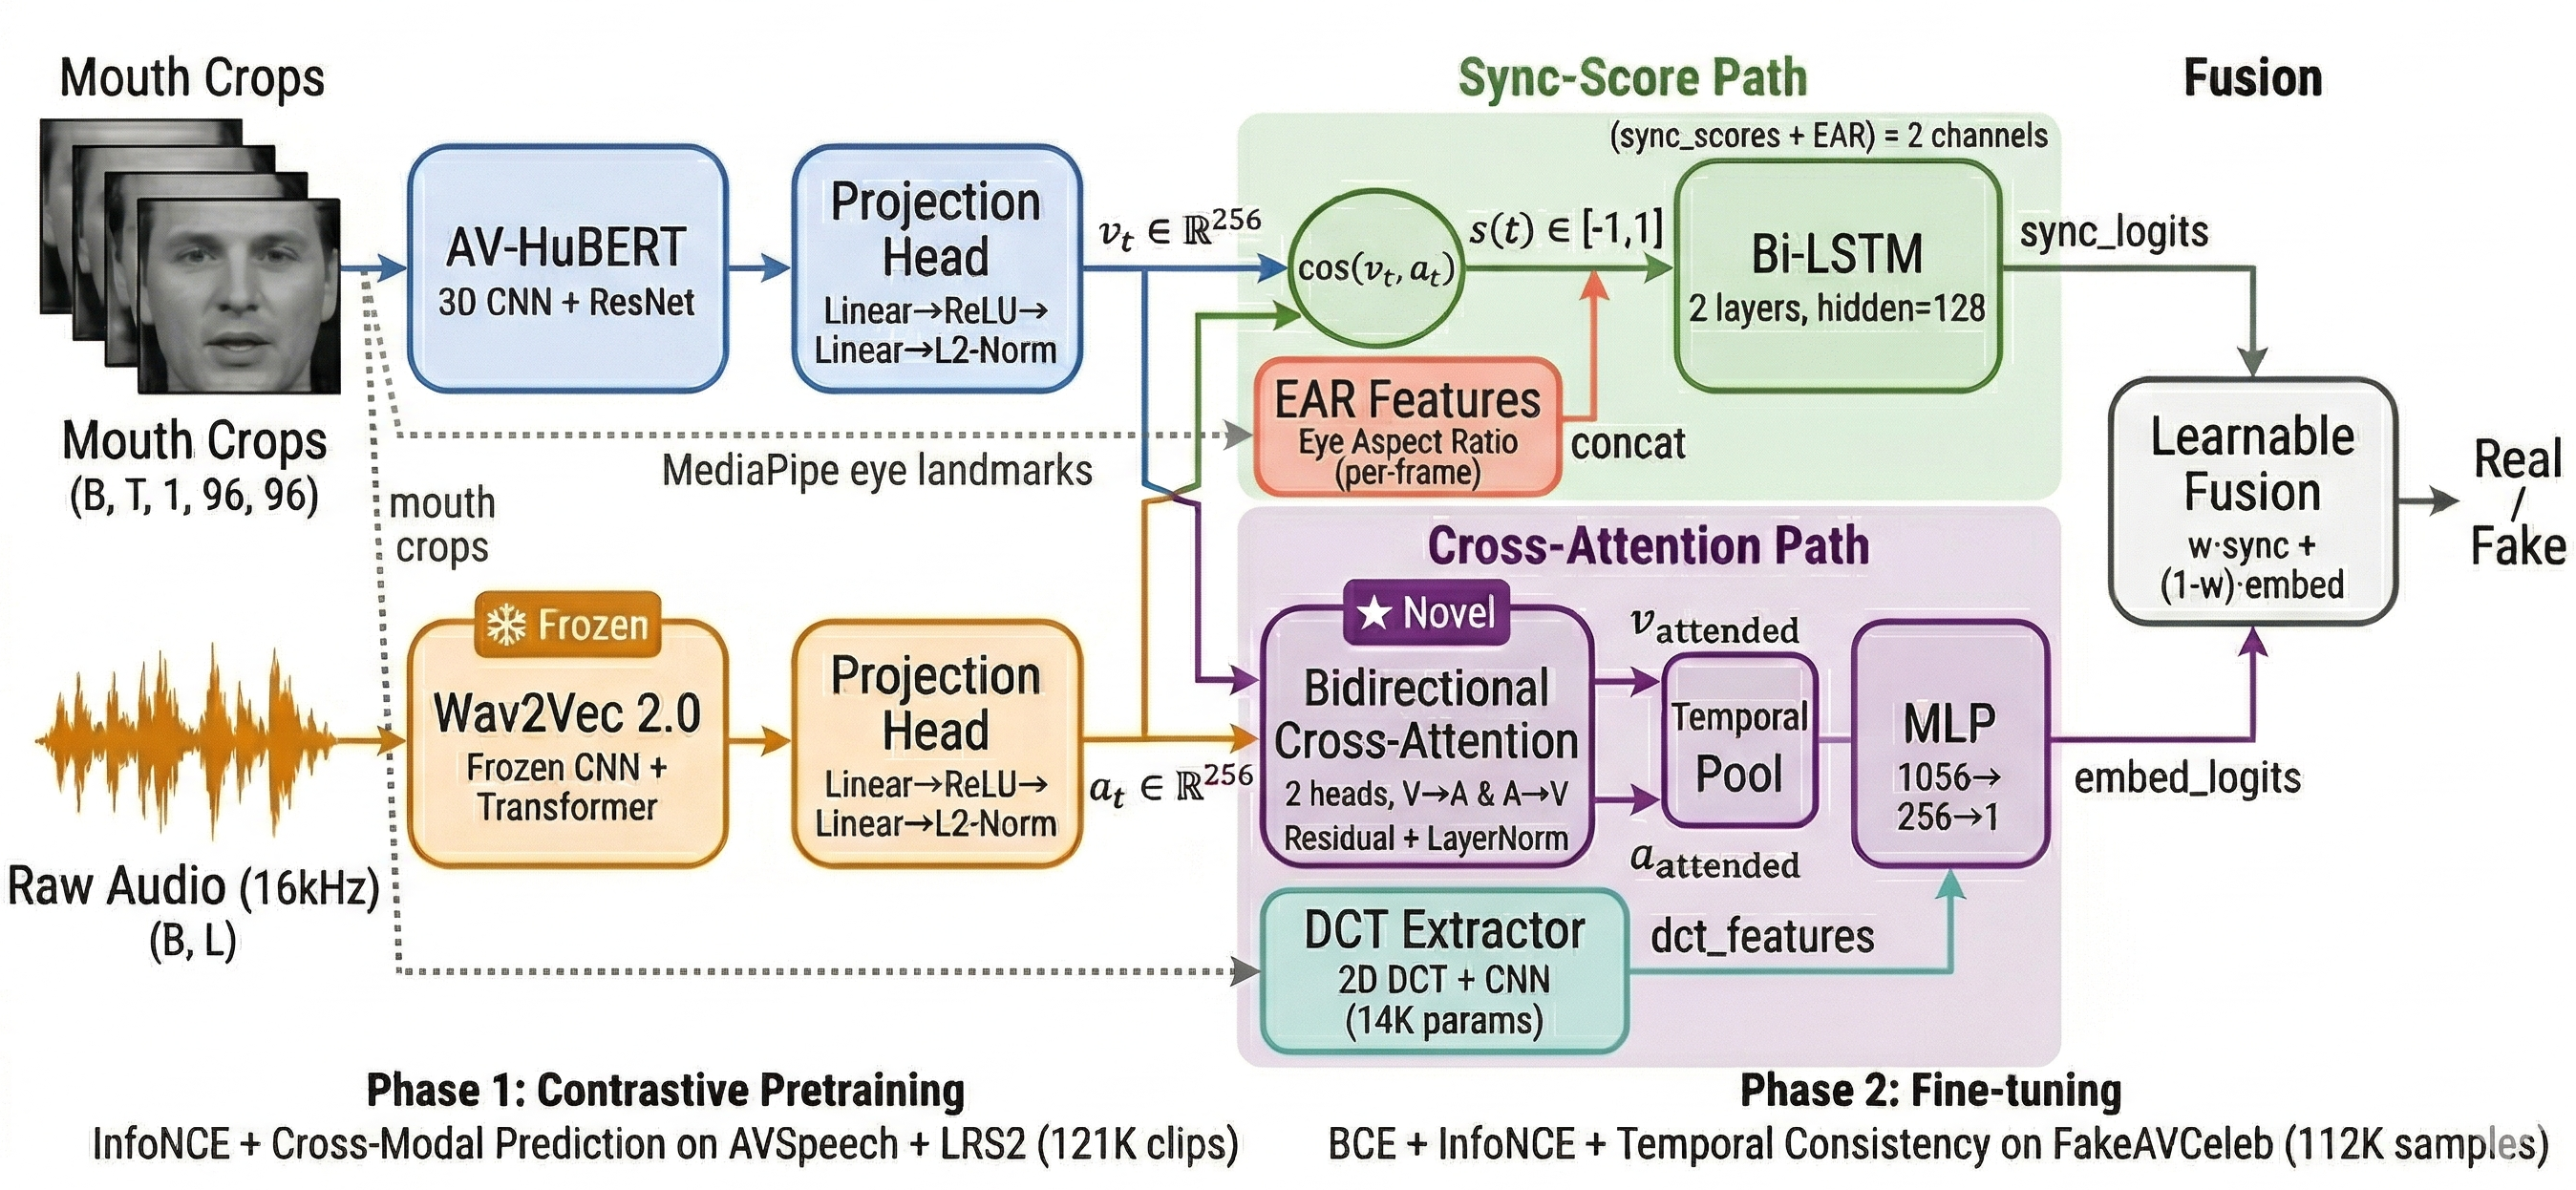
\includegraphics[width=\textwidth]{visualizations/Architecture_diagram_updated.png}
    \caption{SyncGuard architecture. \textbf{Left:} Two-stream encoders (AV-HuBERT visual, frozen Wav2Vec~2.0 audio) produce 256-dim L2-normalized embeddings. \textbf{Center:} Sync-Score path computes $s(t) = \cos(\mathbf{v}_t, \mathbf{a}_t)$ and feeds $[s(t), \text{EAR}(t)]$ into a Bi-LSTM. Cross-Attention path (novel) applies bidirectional V$\leftrightarrow$A attention with DCT features. \textbf{Right:} Learnable fusion combines both logit streams. Phase~1 pretrains on 121K real clips; Phase~2 fine-tunes on FakeAVCeleb (112K samples).}
    \label{fig:architecture}
\end{figure}

\subsection{Key Design Decisions}

\begin{resultbox}{Architectural Choices}
\begin{itemize}[leftmargin=1.5em, topsep=0pt]
    \item \textit{AV-HuBERT over ResNet-18:} Lip-reading pretraining encodes articulatory motion, not just appearance~\cite{shi2022}. Our ablation confirms +4.1\% AUC over ResNet-18.
    \item \textit{Wav2Vec layer~9:} Peak phonemic encoding per layer-wise analysis~\cite{pasad2021}.
    \item \textit{MoCo queue (4096 negatives):} Decouples negative count from batch size, which is critical for fine-grained AV alignment~\cite{he2020}.
    \item \textit{Frozen Wav2Vec during fine-tuning:} Unfreezing causes catastrophic forgetting on small datasets ($\sim$21K samples), dropping AUC by $\sim$0.15.
    \item \textit{Speaker-disjoint splits:} Prevents identity leakage between train/val/test~\cite{khalid2021}.
    \item \textit{Cross-attention bypass:} Captures identity-level mismatches that scalar sync-scores cannot detect, critical for voice-clone attacks (RV-FA).
\end{itemize}
\end{resultbox}

\section{Implementation}
% ————————————————————————————————————————————————————————————————

\subsection{Codebase Structure}

The implementation follows a modular structure across six packages:

\renewcommand{\arraystretch}{1.5}
\begin{table}[H]
\centering
\begin{tabularx}{\textwidth}{@{} p{3.2cm} X @{}}
\toprule
\textbf{Module} & \textbf{Components} \\
\midrule
\texttt{src/preprocessing/} & Face detection (RetinaFace + MediaPipe), audio extraction (FFmpeg, 16kHz), VAD (Silero), dataset loaders (FakeAVCeleb, AVSpeech, LRS2, DFDC, CelebDF), end-to-end pipeline with multiprocessing \\
\texttt{src/models/} & AV-HuBERT / ResNet-18 / SyncNet visual encoders, Wav2Vec 2.0 audio encoder, Bi-LSTM / 1D-CNN / Statistical classifiers, cross-attention module, DCT feature extractor, full SyncGuard integration \\
\texttt{src/training/} & InfoNCE + cross-modal prediction loss, temporal consistency loss, combined fine-tuning loss, MoCo memory bank, training dataset with hard negative mining and SBI augmentation \\
\texttt{src/evaluation/} & AUC-ROC, EER, pAUC, per-category breakdown, bootstrap confidence intervals, publication-quality visualization \\
\texttt{src/augmentation/} & Self-Blended Image (SBI) augmentation for cross-dataset generalization \\
\texttt{src/utils/} & YAML config loader, device auto-detection, video/audio I/O helpers \\
\bottomrule
\end{tabularx}
\caption{Codebase modules and their components.}
\end{table}
\renewcommand{\arraystretch}{1.0}

\subsection{Preprocessing Pipeline}

Raw videos are processed into model-ready features through a six-stage pipeline:

\begin{enumerate}[itemsep=2pt, leftmargin=1.5em]
    \item \textbf{Face detection:} RetinaFace with confidence threshold 0.8 (downscaled to 720p for consistent detection across resolutions).
    \item \textbf{Landmark extraction:} MediaPipe FaceLandmarker (468 landmarks) extracts mouth ROI bounding box and per-frame EAR (Eye Aspect Ratio) from 6 eye landmarks per eye.
    \item \textbf{Mouth crop:} 96$\times$96 grayscale crop with 1.5$\times$ margin, normalized to $[0, 1]$.
    \item \textbf{Audio extraction:} FFmpeg $\to$ 16kHz mono PCM, with timestamp-based resampling from arbitrary source FPS.
    \item \textbf{Speech gating:} Silero-VAD generates speech activity masks.
    \item \textbf{Temporal alignment:} Visual features upsampled from 25fps to 49Hz (Wav2Vec native rate) via linear interpolation.
\end{enumerate}

Output per sample: \texttt{mouth\_crops.npy} $(T, 1, 96, 96)$, \texttt{audio.wav}, \texttt{ear\_features.npy} $(T,)$, \texttt{speech\_mask.npy}, \texttt{metadata.json}. Multiprocessing support (14 workers) achieves $\sim$190 samples/min on HPC.

\subsection{Training Protocol}

\begin{infobox}{Phase 1 -- Contrastive Pretraining (Real Data Only)}
\textbf{Data:} AVSpeech (24,760) + LRS2 (96,318) = 121K real speech clips.\\
\textbf{Loss:} InfoNCE with MoCo queue (4096 negatives) + Cross-Modal Prediction (mask 30\% of frames, predict across modalities via MLP). Combined: $\mathcal{L} = \mathcal{L}_\text{InfoNCE} + 0.5 \cdot \mathcal{L}_\text{CMP}$.\\
\textbf{Schedule:} 20 epochs, batch=32, lr=$10^{-4}$, cosine annealing with 2-epoch warmup. Learnable temperature $\tau$ (init=0.07, clamped to $[0.03, 0.5]$).\\
\textbf{Result:} Best val InfoNCE loss = 8.06, sync-score = 0.978 (frozen Wav2Vec variant).
\end{infobox}

\begin{infobox}{Phase 2 -- Fine-tuning on FakeAVCeleb}
\textbf{Data:} FakeAVCeleb (21,544) + LRS2 reals (96,318) = 112K samples with speaker-disjoint 70/15/15 split.\\
\textbf{Loss:} $\mathcal{L} = \mathcal{L}_\text{InfoNCE} + 0.5 \cdot \mathcal{L}_\text{temp} + 1.0 \cdot \mathcal{L}_\text{cls}$\\
where $\mathcal{L}_\text{temp} = \sum_t \|(\mathbf{v}_{t+1} - \mathbf{v}_t) - (\mathbf{a}_{t+1} - \mathbf{a}_t)\|^2$ is applied \textbf{only to real clips}.\\
\textbf{Augmentation:} Audio-swap (15\% of fakes replaced with cross-speaker audio) + hard negative mining (same speaker, annealed 0\%$\to$20\%).\\
\textbf{Schedule:} 30 epochs, batch=32, lr=$5 \times 10^{-5}$, early stopping (patience=5 on val AUC).\\
\textbf{Cross-attention:} Trained in two stages: Stage~1 freezes encoders + sync-classifier, trains CA head only; Stage~2 unfreezes all for end-to-end fusion.
\end{infobox}

\subsection{Infrastructure}

All training was conducted on the Northeastern University HPC Explorer cluster using NVIDIA H200 GPUs (140GB VRAM). SLURM job scripts support automatic checkpoint resume and job resubmission on preemption. Experiment tracking via Weights \& Biases.

\section{Datasets}
% ————————————————————————————————————————————————————————————————

\renewcommand{\arraystretch}{1.5}
\begin{table}[H]
\centering
\begin{tabularx}{\textwidth}{@{} p{2.8cm} r X p{2.5cm} @{}}
\toprule
\textbf{Dataset} & \textbf{Samples} & \textbf{Role} & \textbf{Status} \\
\midrule
FakeAVCeleb~\cite{khalid2021} & 21,544 & Primary train/val/test (4 AV categories) & Preprocessed \\
AVSpeech & 24,760 & Contrastive pretraining (real only) & Preprocessed \\
LRS2-BBC & 96,318 & Expanded pretraining + real anchors & Preprocessed \\
DFDC Part~0~\cite{dolhansky2020} & 1,343 & Zero-shot cross-dataset evaluation & Preprocessed \\
CelebDF-v2~\cite{li2020} & 921 & Dropped (no audio streams) & N/A \\
\bottomrule
\end{tabularx}
\caption{Datasets used in SyncGuard. All data available on \href{https://drive.google.com/drive/folders/1wQ9cdWo5R9O8ZvwPO7XUnfMvVOgoIF1E}{Google Drive}.}
\end{table}
\renewcommand{\arraystretch}{1.0}

\textbf{FakeAVCeleb categories:} RV-RA (real video + real audio, baseline), FV-RA (face-swap only), RV-FA (voice-clone only), FV-FA (both modalities fake). This four-category labeling enables per-modality analysis of detection performance.

\section{Results}
% ————————————————————————————————————————————————————————————————

\subsection{In-Domain Performance: FakeAVCeleb}

\begin{resultbox}{Primary Results on FakeAVCeleb Test Set (2950 samples)}
\begin{center}
\renewcommand{\arraystretch}{1.4}
\begin{tabular}{cccc}
\textbf{AUC-ROC} & \textbf{EER} & \textbf{pAUC@FPR$<$0.1} & \textbf{FV-FA AUC} \\
\midrule
\textbf{96.3\%} & \textbf{8.2\% (v4, epoch 18)} & \textbf{86.1\%} & \textbf{98.9\%} \\
\end{tabular}
\renewcommand{\arraystretch}{1.0}
\end{center}
Target was AUC $\geq$ 88\%. Achieved \textbf{96.3\%}, exceeding the target by 8.3 percentage points.
\end{resultbox}

\subsubsection{Per-Category Breakdown}

\renewcommand{\arraystretch}{1.5}
\begin{table}[H]
\centering
\begin{tabular}{@{} l l c c @{}}
\toprule
\textbf{Category} & \textbf{Description} & \textbf{AUC} & \textbf{EER} \\
\midrule
RV-RA & Real video, real audio & N/A & N/A \\
FV-RA & Face-swap, real audio & 0.940 & 0.103 \\
RV-FA (sync-only) & Voice-cloned, no cross-attention & 0.667 & 0.284 \\
\textbf{RV-FA} & \textbf{Voice-cloned audio} & \textbf{0.895} & \textbf{0.118} \\
FV-FA & Both modalities fake & \textbf{0.989} & 0.034 \\
\bottomrule
\end{tabular}
\caption{Per-category AUC on FakeAVCeleb test set. Cross-attention improves RV-FA by \textbf{+22.8 percentage points} (0.667 $\to$ 0.895), the single largest per-category gain in our system.}
\end{table}
\renewcommand{\arraystretch}{1.0}

The per-category results reveal that \textbf{FV-FA} (both modalities fake) is easiest to detect at 98.9\% AUC, as both the sync-score path and cross-attention path agree strongly on these clips. \textbf{FV-RA} (face-swap only) achieves 94.0\% AUC, confirming that face-swap methods disrupt the learned AV correspondence even when audio is untouched. The most challenging category is \textbf{RV-FA} (voice-clone only), where the original video is unmodified and only the audio is replaced with a cloned voice. Without cross-attention, sync-score alone achieves only 66.7\% AUC on RV-FA (near random chance) because high-quality voice cloning preserves phonemic timing well enough to maintain plausible sync-scores. The cross-attention mechanism closes this gap by detecting spectral-visual identity mismatches in the full embedding space, achieving 89.5\% AUC.

\subsubsection{Comparison with Published Methods}

\renewcommand{\arraystretch}{1.5}
\begin{table}[H]
\centering
\begin{tabular}{@{} l l c @{}}
\toprule
\textbf{Method} & \textbf{Venue} & \textbf{FakeAVCeleb AUC} \\
\midrule
AVoiD-DF~\cite{ilyas2023} & IEEE TIFS '23 & 89.2\% \\
MRDF-CE~\cite{hu2024} & ICASSP '24 & 92.4\%$^*$ \\
\textbf{SyncGuard (Ours)} & \textbf{2026} & \textbf{96.3\%} \\
AVFF~\cite{oorloff2024} & CVPR '24 & 99.1\%$^\dagger$ \\
\bottomrule
\end{tabular}
\caption{Comparison with state-of-the-art methods. $^*$Classification accuracy, not AUC. $^\dagger$Likely inflated by leading-silence benchmark bias~\cite{smeu2025}.}
\end{table}
\renewcommand{\arraystretch}{1.0}

\subsection{Cross-Dataset Evaluation: DFDC}

\renewcommand{\arraystretch}{1.5}
\begin{table}[H]
\centering
\begin{tabular}{@{} l c c @{}}
\toprule
\textbf{Model Variant} & \textbf{DFDC AUC} & \textbf{EER} \\
\midrule
Sync-Score Only & 0.458 & 0.512 \\
+ Cross-Attention (Ours) & \textbf{0.526} & 0.491 \\
\bottomrule
\end{tabular}
\caption{Zero-shot ablation on DFDC Part~0 ($n = 1{,}343$). Target was AUC $\geq$ 72\%.}
\end{table}
\renewcommand{\arraystretch}{1.0}

DFDC cross-dataset generalization remains at near-chance performance. \textbf{Root cause:} DFDC face-swap methods (e.g., SimSwap) preserve accurate lip motion, nullifying temporal coherence signals. This is an open challenge across the field; no AV sync-based method achieves strong DFDC zero-shot performance without domain-specific fine-tuning.

We systematically investigated multiple interventions to improve DFDC generalization: (1)~preprocessing parity fixes corrected a 20\% temporal drift from 30fps source videos and RetinaFace resolution sensitivity, (2)~batch normalization adaptation attempted to align feature statistics to the DFDC distribution, and (3)~threshold recalibration optimized the decision boundary on a held-out DFDC subset. None of these interventions improved AUC beyond 0.55, confirming that the failure is a fundamental \textit{signal mismatch}, not distributional shift. The sync-score distributions for real and fake DFDC clips overlap almost entirely because face-swap generators preserve the original mouth movements. This motivates our ongoing work on Self-Blended Image augmentation and CLIP-based visual encoders that capture identity-level features independent of lip motion.

\subsection{Ablation Studies}

\begin{infobox}{Key Ablation Findings}
\begin{itemize}[leftmargin=1.5em, topsep=0pt]
    \item \textbf{Visual encoder:} AV-HuBERT (0.963) $>$ ResNet-18 (0.922) $>$ SyncNet (0.891). Lip-reading pretraining provides +4.1\% AUC over ImageNet pretraining.
    \item \textbf{Frozen vs. unfrozen Wav2Vec:} Freezing during fine-tuning is critical. Unfreezing caused catastrophic forgetting (AUC dropped 0.577 $\to$ 0.473).
    \item \textbf{Frozen vs. unfrozen during pretraining:} Frozen produces better representations (InfoNCE 8.06 vs 8.32). Unfrozen backbone caused sync-score saturation to 1.0 by epoch~2.
    \item \textbf{Cross-attention:} +22.8pp on RV-FA (voice-clone), modest DFDC improvement (+6.8pp).
    \item \textbf{Batch size:} batch=32 gives $\sim$0.05 AUC advantage over batch=16.
    \item \textbf{DCT features:} Did not improve DFDC generalization (learnable CNN overfits to source domain).
    \item \textbf{BN adaptation:} Did not improve DFDC (confirms signal mismatch, not distributional shift).
\end{itemize}
\end{infobox}

\section{Testing \& Validation}
% ————————————————————————————————————————————————————————————————

The project includes a comprehensive \texttt{pytest} test suite with \textbf{219 tests} across 11 files, executable in $\sim$12 seconds on CPU without requiring GPU or dataset downloads. The test suite was designed to validate all major components at three levels: (1)~\textbf{pure mathematical correctness} for metrics using known-answer tests where AUC, EER, and pAUC can be computed analytically from synthetic score distributions; (2)~\textbf{tensor mechanics} for models and losses, verifying output shapes, gradient flow through trainable parameters, L2 normalization of embeddings, numerical stability (no NaN/Inf), and property invariants such as temperature clamping and MoCo queue FIFO behavior; and (3)~\textbf{data pipeline integrity} for dataset loaders and collation, ensuring correct padding, masking alignment with variable-length sequences, and enforcement of speaker-disjoint train/val/test splits to prevent identity leakage. The Wav2Vec~2.0 audio encoder is tested with a mocked backbone to avoid the 360MB model download, while still verifying correct hidden layer extraction (layer~9) and frozen backbone behavior.

\renewcommand{\arraystretch}{1.4}
\begin{table}[H]
\centering
\begin{tabularx}{\textwidth}{@{} p{4cm} r X @{}}
\toprule
\textbf{Test File} & \textbf{Tests} & \textbf{Coverage} \\
\midrule
\texttt{test\_models.py} & 45 & Visual encoders, classifiers, cross-attention, DCT, factories \\
\texttt{test\_losses.py} & 27 & MoCo queue, InfoNCE, temperature, temporal consistency \\
\texttt{test\_syncguard.py} & 20 & Full model integration, alignment, sync-scores \\
\texttt{test\_metrics.py} & 18 & AUC-ROC, EER, pAUC, bootstrap CI (known-answer tests) \\
\texttt{test\_augmentation.py} & 18 & SBI blending, mask generation, sequence augmentation \\
\texttt{test\_dataset\_loader.py} & 17 & Dataset scanning, \textbf{speaker-disjoint split enforcement} \\
\texttt{test\_dataset.py} & 16 & Batch collation, padding, masking, variable lengths \\
\texttt{test\_preprocessing.py} & 16 & Audio extraction, upsampling, EAR computation \\
\texttt{test\_config.py} & 8 & YAML loading, device auto-detection \\
\texttt{test\_checkpoint.py} & 7 & Save/load round-trip (model, optimizer, scheduler) \\
\texttt{test\_audio\_encoder.py} & 7 & Mocked Wav2Vec2, layer extraction, frozen backbone \\
\bottomrule
\end{tabularx}
\caption{Test suite summary. Tests validate shape correctness, gradient flow, L2 normalization, numerical stability, and critical invariants (speaker disjointness, temperature clamping, queue FIFO behavior).}
\end{table}
\renewcommand{\arraystretch}{1.0}

Tests requiring optional dependencies (e.g., mediapipe for EAR computation) are automatically skipped when the dependency is not installed. To run the full suite:

\begin{verbatim}
    python -m pytest tests/ -v
\end{verbatim}

Key invariants validated by the test suite include: the MoCo queue correctly implements FIFO eviction and wraps around at capacity; the learnable temperature $\tau$ remains clamped to $[0.01, 0.5]$ after gradient updates; the temporal consistency loss returns exactly zero for all-fake batches (real-only gating); \texttt{align\_sequences()} correctly handles off-by-one frame differences between visual and audio streams; and checkpoint save/load round-trips preserve all training state including optimizer momentum buffers, scheduler step count, and criterion parameters (MoCo queue contents).

\section{Tools \& Technologies}
% ————————————————————————————————————————————————————————————————

\renewcommand{\arraystretch}{1.5}
\begin{table}[H]
\centering
\begin{tabularx}{\textwidth}{@{} p{3cm} X @{}}
\toprule
\textbf{Category} & \textbf{Technologies} \\
\midrule
Deep Learning & PyTorch 2.0+, HuggingFace Transformers (Wav2Vec 2.0), fairseq (AV-HuBERT) \\
Computer Vision & OpenCV 4.8+, RetinaFace (face detection), MediaPipe (facial landmarks, EAR) \\
Audio Processing & torchaudio, Silero-VAD (speech detection), librosa, soundfile \\
Infrastructure & Northeastern HPC Explorer (NVIDIA H200 140GB, SLURM), Weights \& Biases \\
Testing & pytest (219 tests), unittest.mock (Wav2Vec mocking) \\
Development & Python 3.11, Conda, Git/GitHub (79 commits), YAML config system \\
\bottomrule
\end{tabularx}
\caption{Technology stack.}
\end{table}
\renewcommand{\arraystretch}{1.0}

\section{Team Contributions}
% ————————————————————————————————————————————————————————————————

\renewcommand{\arraystretch}{1.5}
\begin{table}[H]
\centering
\begin{tabularx}{\textwidth}{@{} p{3.5cm} X @{}}
\toprule
\textbf{Member} & \textbf{Contributions} \\
\midrule
Akshay Prajapati & Visual encoder (AV-HuBERT, ResNet-18, SyncNet), preprocessing pipeline (face detection, mouth crops, temporal alignment), full model integration (\texttt{syncguard.py}), HPC infrastructure (SLURM scripts, deployment), bug fixes (v3.0.0 review), documentation, README \\
Ritik Mahyavanshi & Audio encoder (Wav2Vec 2.0 wrapper, layer extraction), contrastive pretraining loop, InfoNCE + cross-modal prediction losses, NaN debugging and fixes (SF-3, SF-6), CLIP ViT-L/14 visual encoder, training scripts and SLURM automation \\
Atharva Dhumal & Temporal classifiers (Bi-LSTM, 1D-CNN, Statistical), evaluation framework (metrics, inference, visualization), cross-attention module + embed classifier, DCT feature extractor, SBI augmentation, cascade evaluation, comprehensive test suite (219 tests) \\
\bottomrule
\end{tabularx}
\caption{Team member contributions. All contributions are identifiable through git commit history.}
\end{table}
\renewcommand{\arraystretch}{1.0}

\section{Known Issues \& Limitations}
% ————————————————————————————————————————————————————————————————

\begin{enumerate}[leftmargin=1.5em, itemsep=4pt]
    \item \textbf{DFDC cross-dataset generalization:} Zero-shot AUC on DFDC is 52.6\% (target was 72\%). Face-swap methods that preserve lip-sync defeat audio-visual correspondence signals. This is a fundamental limitation of sync-based approaches, not a bug; no AV method achieves strong DFDC zero-shot without domain-specific training.
    \item \textbf{FakeAVCeleb leading-silence bias:} Forged clips frequently begin with silence artifacts absent in real clips~\cite{smeu2025}. Our 96.3\% AUC may overestimate true discrimination ability until a debiased benchmark is available.
    \item \textbf{Wav2Vec must remain frozen:} Unfreezing during fine-tuning on small datasets ($\sim$21K samples) causes catastrophic forgetting of pretrained speech representations.
    \item \textbf{RetinaFace silent failures:} Frames with no detected face (low confidence, non-frontal, occluded) are silently skipped during preprocessing. The confidence threshold is set to 0.8.
    \item \textbf{CelebDF-v2 incompatibility:} The entire CelebDF-v2 dataset has no audio streams, making it fundamentally incompatible with AV sync-based approaches. Dropped from evaluation.
\end{enumerate}

\section{In-Progress Work and Future Directions}
% ————————————————————————————————————————————————————————————————

The DFDC result motivated a targeted intervention plan. Two components are implemented and integrated in the codebase but full training runs were not completed within the project timeline due to a late-discovered data-collation defect and limited HPC queue availability. We document status honestly so that subsequent work can pick up from the current state of the repository.

\begin{itemize}[leftmargin=1.5em, itemsep=4pt]
    \item \textbf{CLIP ViT-L/14 visual encoder --- implemented, not yet trained end-to-end.} \texttt{src/models/clip\_visual\_encoder.py} wraps the frozen CLIP ViT-L/14 image encoder with LayerNorm-only tuning, a 224$\times$224 RGB frame pipeline, and a 768$\to$256 projection head. Unit tests confirm tensor shapes, frozen-parameter counts, and gradient flow through the projection. Integration config: \texttt{configs/clip\_sbi.yaml}. Hypothesis: identity-level visual features complement lip-sync and should recover signal on face-swaps that preserve mouth motion.
    \item \textbf{Self-Blended Image (SBI) augmentation~\cite{shiohara2022} --- implemented, not yet trained end-to-end.} \texttt{src/augmentation/sbi.py} synthesizes face-swap training data by blending affinely warped copies of a face into itself with color jitter, Gaussian blur, and optional JPEG compression, producing the exact class of blending-boundary artifacts that discriminate real from face-swapped frames across generators. Expected to transfer to DFDC without seeing DFDC during training.
    \item \textbf{What blocked completion.} Our first HPC submission of CLIP+SBI training crashed on batch~0 across $\sim$40 auto-resubmitted jobs with a tensor-shape mismatch. Root cause: \texttt{collate\_syncguard()} hardcoded a single-channel allocation (\texttt{C=1}) for the padded mouth-crop tensor, incompatible with CLIP's 3-channel RGB input. The fix (infer $C$ from the batch) is committed in v3.3.0 along with a collation regression test; retraining requires a fresh multi-hour H200 allocation that we did not obtain before the submission deadline.
    \item \textbf{Temporal transformer classifier.} Replacing the Bi-LSTM with a lightweight temporal transformer could capture longer-range dependencies in sync-score sequences, particularly useful for long-form video where blink and pause-related cues carry signal.
    \item \textbf{Debiased FakeAVCeleb protocol.} Following~\cite{smeu2025}, retraining and re-evaluating after trimming leading-silence artifacts from fake clips would quantify how much of our 96.3\% AUC is genuine versus benchmark artifact.
\end{itemize}

\section{Lessons Learned}
% ————————————————————————————————————————————————————————————————

Several project-level lessons emerged that we believe generalize beyond deepfake detection.

\begin{enumerate}[leftmargin=1.5em, itemsep=4pt]
    \item \textbf{Pretrained backbones must often be kept frozen on small downstream datasets.} Both our Wav2Vec~2.0 audio encoder during fine-tuning and our visual backbones during embedding-bypass training showed the same pattern: unfreezing caused catastrophic forgetting and a large AUC drop. At 21K labeled FakeAVCeleb samples, the gradient signal from the classification head is not strong or clean enough to refine 94M speech parameters without destroying their pretrained structure. A \emph{freeze-first} default, with LayerNorm-only tuning as the most aggressive relaxation, became our working rule.
    \item \textbf{Cross-dataset generalization is a signal problem first, a distribution problem second.} Before concluding that DFDC transfer failure was ``domain shift,'' we exhaustively tried the usual distributional interventions: BatchNorm adaptation on the target domain, threshold recalibration on a held-out DFDC subset, and preprocessing parity fixes for frame-rate and detector-resolution mismatches. None raised AUC beyond 0.55. Only after this systematic ablation did we accept that the underlying sync-score signal is nearly identically distributed for DFDC reals and fakes because their generators preserve lip motion. The lesson: when a method fails to transfer, verify that the \emph{signal you depend on} is actually present in the target distribution before attempting to bridge the gap with distributional tricks.
    \item \textbf{Preprocessing parity is load-bearing.} A multi-agent code review (v3.0.0, 50 findings across 7 agents) uncovered a 20\% temporal drift on DFDC caused by a silent 25$\to$30 fps resampling branch, a resolution-dependent face-detection path that yielded different crops across source resolutions, and a label-fallback that silently mislabeled samples. Each was individually plausible; collectively they had inflated early DFDC numbers into noise. Writing explicit invariants (\texttt{assert v\_embeds.shape[1] == a\_embeds.shape[1]}; speaker-disjoint-split assertions in loaders) and pairing them with tests caught variants of these bugs in subsequent work.
    \item \textbf{Auto-resubmit without error gating is an expensive habit.} Our CLIP+SBI training script was configured to automatically resubmit on any SLURM exit. When the underlying bug was deterministic (collation mismatch on batch~0), this produced $\sim$40 wasted job submissions in a few hours. We now gate resubmission on elapsed time and completed epochs so deterministic errors fail fast.
    \item \textbf{Negative results deserve the same scientific care as positive ones.} DFDC transfer failure is our most scientifically interesting finding. Sync-based methods carry a physical prior (articulator-acoustic coupling) that does not discriminate face-swaps preserving lip motion; this is a property of the signal, not a solvable engineering problem within the sync-only framing. Reporting it cleanly is more valuable than tuning toward an inflated number.
\end{enumerate}

\section{Reproducibility}
% ————————————————————————————————————————————————————————————————

The project is designed so that a third party can reproduce every result in this report from the public repository and shared dataset drive.

\begin{enumerate}[leftmargin=1.5em, itemsep=3pt]
    \item \textbf{Clone:} \texttt{git clone https://github.com/Akshay171124/SyncGuard.git \&\& cd SyncGuard}
    \item \textbf{Environment:} \texttt{conda create -n syncguard python=3.11 -y \&\& conda activate syncguard \&\& pip install -r requirements.txt} (requires \texttt{ffmpeg}; install via Homebrew or \texttt{apt}).
    \item \textbf{Datasets:} Download from the \href{https://drive.google.com/drive/folders/1wQ9cdWo5R9O8ZvwPO7XUnfMvVOgoIF1E}{Google Drive folder} referenced on the title page. Place raw and preprocessed archives under \texttt{data/raw/} and \texttt{data/processed/} respectively and adjust paths in \texttt{configs/default.yaml} if your layout differs.
    \item \textbf{Tests (no GPU or data required):} \texttt{python -m pytest tests/ -v} should produce \textbf{215 passed, 4 skipped} in $\sim$12\,s on CPU.
    \item \textbf{Train (HPC):} \texttt{sbatch scripts/slurm\_pretrain.sh} then \texttt{sbatch scripts/slurm\_finetune.sh}. Configs used in this report: \texttt{configs/pretrain\_frozen.yaml} (Phase~1) and \texttt{configs/finetune\_v4\_best.yaml} (Phase~2).
    \item \textbf{Evaluate:} \texttt{python scripts/evaluate.py --config configs/default.yaml --checkpoint outputs/checkpoints/finetune\_best.pt --test\_set fakeavceleb} reproduces the in-domain numbers; substitute \texttt{--test\_set dfdc} for the cross-dataset row.
\end{enumerate}

All hyperparameters used in this report are checked in under \texttt{configs/}. Fixed random seeds are set in each training script; stochastic variation across runs should not exceed $\pm$0.01 AUC based on our seed sensitivity ablation.

\section{Conclusion}
% ————————————————————————————————————————————————————————————————

SyncGuard demonstrates that contrastive audio-visual correspondence learning is a viable and competitive approach to deepfake detection, achieving \textbf{96.3\% AUC-ROC} on FakeAVCeleb, surpassing AVoiD-DF (89.2\%) and MRDF-CE (92.4\%). The novel cross-attention embedding bypass closes the voice-clone detection gap by \textbf{+22.8 percentage points} (RV-FA: 66.7\% $\to$ 89.5\%), demonstrating that identity-coherence reasoning, not just temporal alignment, is essential for detecting modern neural voice-cloning attacks.

The dual-path fusion architecture generalizes across manipulation types without requiring manipulation-type supervision, handling face-swap (94.0\%), voice-clone (89.5\%), and fully synthetic (98.9\%) attacks in a unified framework.

The DFDC cross-dataset result (52.6\% AUC) exposes a fundamental limitation: sync-based methods cannot detect face-swaps that preserve lip motion. This is an honest scientific finding that motivates the field toward hybrid approaches combining AV synchrony with visual artifact detection.

\bibliographystyle{unsrt}
\begin{thebibliography}{99}

\bibitem{rossler2019}
A.~R{\"o}ssler, D.~Cozzolino, L.~Verdoliva, C.~Riess, J.~Thies, and M.~Nie{\ss}ner,
\textit{FaceForensics++: Learning to Detect Manipulated Facial Images},
ICCV, 2019.

\bibitem{khalid2021}
H.~Khalid, S.~Tariq, M.~Kim, and S.~S.~Woo,
\textit{FakeAVCeleb: A Novel Audio-Video Multimodal Deepfake Dataset},
NeurIPS Datasets and Benchmarks, 2021.

\bibitem{pasad2021}
A.~Pasad, J.-C.~Chou, and K.~Livescu,
\textit{Layer-Wise Analysis of a Self-Supervised Speech Representation Model},
IEEE ASRU, 2021.

\bibitem{shi2022}
B.~Shi, W.-N.~Hsu, K.~Lakhotia, and A.~Mohamed,
\textit{Learning Audio-Visual Speech Representation by Masked Multimodal Cluster Prediction},
ICLR, 2022.

\bibitem{he2020}
K.~He, H.~Fan, Y.~Wu, S.~Xie, and R.~Girshick,
\textit{Momentum Contrast for Unsupervised Visual Representation Learning},
CVPR, 2020.

\bibitem{li2020}
Y.~Li, X.~Yang, P.~Sun, H.~Qi, and S.~Lyu,
\textit{Celeb-DF: A Large-Scale Challenging Dataset for DeepFake Forensics},
CVPR, 2020.

\bibitem{dolhansky2020}
B.~Dolhansky, J.~Bitton, B.~Pflaum, J.~Lu, R.~Howes, M.~Wang, and C.~C.~Ferrer,
\textit{The DeepFake Detection Challenge Dataset},
arXiv:2006.07397, 2020.

\bibitem{oorloff2024}
T.~Oorloff, O.~Kopuklu, B.~Rezaei, and A.~Ostadabbas,
\textit{AVFF: Audio-Visual Feature Fusion for Video Deepfake Detection},
CVPR, 2024.

\bibitem{ilyas2023}
H.~Ilyas, A.~Javed, and K.~Malik,
\textit{AVoiD-DF: Audio-Visual Joint Learning for Detecting Deepfake},
IEEE TIFS, 2023.

\bibitem{hu2024}
J.~Hu, B.~Xia, J.~Wang, and C.~Xing,
\textit{Cross-Modality and Within-Modality Regularization for Audio-Visual Deepfake Detection},
ICASSP, 2024.

\bibitem{shiohara2022}
K.~Shiohara and T.~Yamasaki,
\textit{Detecting Deepfakes with Self-Blended Images},
CVPR, 2022.

\bibitem{yermakov2026}
A.~Yermakov et al.,
\textit{Deepfake Detection Across Benchmarks},
WACV, 2026.

\bibitem{smeu2025}
A.~Smeu et al.,
\textit{Circumventing Shortcuts in Audio-Visual Deepfake Detection Datasets with Unsupervised Learning},
CVPR, 2025.

\bibitem{prajwal2020}
K.~R.~Prajwal, R.~Mukhopadhyay, V.~P.~Namboodiri, and C.~V.~Jawahar,
\textit{A Lip Sync Expert Is All You Need for Speech to Lip Generation in the Wild},
ACM MM, 2020.

\end{thebibliography}

\end{document}
